% Provenance (never printed): see sources/outline_sources.md and sources/book1/BRIEFS.md (g7/04).
\chapter{How a Processor Runs a Program}\label{ch:g7:how-a-processor-runs-a-program}

A \omterm{def:g3:inside-the-computer:processor}{processor} understands neither Python nor English. It is a chip of silicon
that can do a few very simple things, very fast. So how does \code{3 + 4}
become 7 inside it? This chapter opens the \omterm{def:g3:inside-the-computer:processor}{processor} of a small \omterm{def:g1:what-is-a-computer:computer}{computer},
the \emph{toy machine} of this series, and follows it step by step.

\begin{recall}
The \omterm{def:g3:inside-the-computer:processor}{processor} carries out \omterm{def:g1:instructions-in-order:instruction}{instructions}, and the \omterm{def:g3:inside-the-computer:memory}{memory} holds the \omterm{def:g4:programs-and-operating-system:program}{programs} and
the data it works on (\cref{ch:g3:inside-the-computer}); \omterm{def:g3:inside-the-computer:memory}{memory} is counted in
\omterm{def:g4:memory-and-storage:byte}{bytes} (\cref{ch:g4:memory-and-storage}). A \omterm{def:g4:memory-and-storage:byte}{byte} is eight \omterm{def:g5:bits-and-bytes:bit}{bits} and holds a
whole number from 0 to 255 (\cref{ch:g5:bits-and-bytes}). Python \omterm{def:g4:programs-and-operating-system:program}{programs} are
carried out by an \omterm{def:g6:first-python-program:interpreter}{interpreter} (\cref{ch:g6:first-python-program}), and a \omterm{def:g4:algorithms-repeat-and-decide:loop}{loop}
goes back to repeat its block (\cref{ch:g6:while-loops}).
\end{recall}

\section{Instructions are numbers in memory}

\begin{definition}[Memory cell and memory address]\label{def:g7:how-a-processor-runs-a-program:cell}\label{def:g7:how-a-processor-runs-a-program:address}
The \omterm{def:g3:inside-the-computer:memory}{memory} is a long row of \emph{memory cells}\index{memory cell}, each
holding one \omterm{def:g4:memory-and-storage:byte}{byte}. The cells are numbered from 0; the number of a cell is its
\emph{memory address}\index{memory address}.
\end{definition}

The toy machine has 256 \omterm{def:g7:how-a-processor-runs-a-program:cell}{memory cells}, with addresses 0 to 255. A real
\omterm{def:g1:what-is-a-computer:computer}{computer} has billions, but they work the same way. The \omterm{def:g4:programs-and-operating-system:program}{program} and its data
sit side by side in that same \omterm{def:g3:inside-the-computer:memory}{memory}: the \omterm{def:g1:instructions-in-order:instruction}{instructions} themselves are
numbers.

\begin{definition}[Machine instruction and machine language]\label{def:g7:how-a-processor-runs-a-program:machine-instruction}
A \emph{machine instruction}\index{machine instruction} is one \omterm{def:g1:instructions-in-order:instruction}{instruction}
that the \omterm{def:g3:inside-the-computer:processor}{processor} carries out directly, written as numbers in \omterm{def:g3:inside-the-computer:memory}{memory}. The
\omterm{def:g1:instructions-in-order:instruction}{instructions} a \omterm{def:g3:inside-the-computer:processor}{processor} understands, with their numbers, are its
\emph{machine language}\index{machine language}.
\end{definition}

Every toy \omterm{def:g1:instructions-in-order:instruction}{instruction} takes two \omterm{def:g4:memory-and-storage:byte}{bytes}. The first holds the number of the
operation, its \emph{operation code}, together with the number of a
\omterm{def:g7:how-a-processor-runs-a-program:register}{register} (next section): the \omterm{def:g4:memory-and-storage:byte}{byte} is $4 \times \text{code} + \text{register}$.
The second \omterm{def:g4:memory-and-storage:byte}{byte} is a number, an address or a second \omterm{def:g7:how-a-processor-runs-a-program:register}{register}. People write
\omterm{def:g1:instructions-in-order:instruction}{instructions} with short names instead of numbers; this chapter uses nine of
them.

\begin{center}
\small
\begin{tabular}{|r|l|l|}
\hline
code & written & what it does \\
\hline
0 & \code{HALT} & stop \\
1 & \code{LOADI R, n} & put the number $n$ in \omterm{def:g7:how-a-processor-runs-a-program:register}{register} \code{R} \\
4 & \code{ADD R, S} & \code{R} becomes \code{R + S} \\
5 & \code{SUB R, S} & \code{R} becomes \code{R - S}; notes whether the result is zero \\
13 & \code{CMP R, S} & computes \code{R - S} only to note whether it is zero or negative \\
16 & \code{JNZ a} & if the last result was not zero, jump to address $a$ \\
17 & \code{JN a} & if the last result was negative, jump to address $a$ \\
19 & \code{IN R} & read a number typed by the user into \code{R} \\
20 & \code{OUT R} & print the number in \code{R} \\
\hline
\end{tabular}
\end{center}

\section{Registers and the program counter}

\begin{definition}[Register]\label{def:g7:how-a-processor-runs-a-program:register}
A \emph{register}\index{register} is a small \omterm{def:g3:inside-the-computer:storage}{storage} place inside the
\omterm{def:g3:inside-the-computer:processor}{processor}, where it keeps the numbers it is working on.
\end{definition}

\begin{definition}[Program counter]\label{def:g7:how-a-processor-runs-a-program:pc}
The \emph{program counter}\index{program counter} is a \omterm{def:g7:how-a-processor-runs-a-program:register}{register} that holds the
address of the next \omterm{def:g1:instructions-in-order:instruction}{instruction} to carry out.
\end{definition}

The toy machine has four \omterm{def:g7:how-a-processor-runs-a-program:register}{registers}, \code{R0} to \code{R3}, of one \omterm{def:g4:memory-and-storage:byte}{byte} each,
and a \omterm{def:g7:how-a-processor-runs-a-program:pc}{program counter}, \code{PC}, which starts at 0. Three \omterm{def:g5:bits-and-bytes:bit}{one-bit}
\emph{flags} remember things about the last result; this chapter only needs
\code{Z}, which is 1 when the last result was zero.

\begin{omfigure}
\begin{tikzpicture}[x=1cm, y=1cm, font=\footnotesize]
  \draw[rounded corners, thick, fill=ocBlue!8] (0,0) rectangle (4.4,4.2);
  \node[font=\small\bfseries] at (2.2,3.85) {processor};
  \foreach \r [count=\i from 0] in {R0,R1,R2,R3} {
    \node[draw=black!60, fill=white, minimum width=1.4cm, minimum height=0.5cm] at (1.5,3.1-0.65*\i) {};
    \node[anchor=east] at (0.75,3.1-0.65*\i) {\texttt{\r}};
  }
  \node[draw=black!60, fill=ocYellow!30, minimum width=1.2cm, minimum height=0.5cm] at (3.3,3.1) {};
  \node at (3.3,2.65) {\code{PC}};
  \node[draw=black!60, fill=white, minimum width=1.2cm, minimum height=0.5cm, font=\scriptsize] at (3.3,1.8) {Z\;N\;C};
  \node at (3.3,1.35) {flags};
  \node[draw=black!60, fill=ocMint!30, minimum width=3.6cm, minimum height=0.45cm] at (2.2,0.35) {fetch, decode, execute};
  \foreach \a in {0,...,15} {
    \pgfmathtruncatemacro{\row}{\a/4}\pgfmathtruncatemacro{\col}{mod(\a,4)}
    \draw[black!60, fill=ocYellow!15] (7+1.0*\col,3.3-0.9*\row) rectangle ++(1.0,0.5);
    \node[font=\scriptsize, ocRed!80!black] at (7.5+1.0*\col,3.98-0.9*\row) {\a};
  }
  \node[font=\small\bfseries] at (9,4.5) {memory};
  \node at (9,0.2) {\dots\ up to cell 255};
  \draw[{Stealth[length=2mm]}-{Stealth[length=2mm]}, very thick, black!60] (4.5,2.1) -- node[above] {bytes} (6.9,2.1);
\end{tikzpicture}

{\small The toy machine: a \omterm{def:g3:inside-the-computer:processor}{processor} with four \omterm{def:g7:how-a-processor-runs-a-program:register}{registers}, a \omterm{def:g7:how-a-processor-runs-a-program:pc}{program counter}
and flags; a \omterm{def:g3:inside-the-computer:memory}{memory} of 256 cells (the first 16 drawn, with their addresses in
red). \omterm{def:g4:memory-and-storage:byte}{Bytes} travel between the two.}
\end{omfigure}

Here is a first \omterm{def:g4:programs-and-operating-system:program}{program}. A \code{;} starts a \omterm{def:g6:first-python-program:comment}{comment}, as \texttt{\#} does in
Python.

\Needspace*{9\baselineskip}
\omcode{code/grade-7/04-how-a-processor-runs-a-program/listings/add_two.toy}{1}{6}{Adding
two numbers on the toy machine.}\label{lst:g7:how-a-processor-runs-a-program:add-two}

Given 3 and 4 to read, it prints 7. In \omterm{def:g3:inside-the-computer:memory}{memory}, these five \omterm{def:g1:instructions-in-order:instruction}{instructions} are
ten \omterm{def:g4:memory-and-storage:byte}{bytes}, from address 0 to address 9. A short Python \omterm{def:g4:programs-and-operating-system:program}{program}, using the
book's toy machine as a module, shows them in decimal and in \omterm{def:g5:bits-and-bytes:binary}{binary}:

\Needspace*{9\baselineskip}
\omcode{code/grade-7/04-how-a-processor-runs-a-program/listings/encode.py}{1}{6}{The
\omterm{def:g4:memory-and-storage:byte}{bytes} of \cref{lst:g7:how-a-processor-runs-a-program:add-two}.}\label{lst:g7:how-a-processor-runs-a-program:encode}

\Needspace*{9\baselineskip}
\omoutput{code/grade-7/04-how-a-processor-runs-a-program/outputs/encode.txt}{Address,
the two \omterm{def:g4:memory-and-storage:byte}{bytes} in decimal, then in \omterm{def:g5:bits-and-bytes:binary}{binary}.}\label{out:g7:how-a-processor-runs-a-program:encode}

\code{IN R0} is $4 \times 19 + 0 = 76$, \code{IN R1} is 77, \code{ADD R0, R1}
is $4 \times 4 + 0 = 16$ followed by the second \omterm{def:g7:how-a-processor-runs-a-program:register}{register}, 1; \code{HALT} is two
zeros.

\begin{omfigure}
\begin{tikzpicture}[x=1cm, y=1cm, font=\footnotesize]
  \foreach \b [count=\i from 0] in {76,0,77,0,16,1,80,0,0,0} {
    \draw[black!60, fill=ocYellow!20] (1.1*\i,0) rectangle ++(1.1,0.7);
    \node[font=\ttfamily] at (1.1*\i+0.55,0.35) {\b};
    \node[ocRed!80!black, font=\scriptsize] at (1.1*\i+0.55,-0.25) {\i};
  }
  \foreach \t [count=\i from 0] in {IN R0, IN R1, {ADD R0, R1}, OUT R0, HALT} {
    \draw[ocBlue, thick, decorate, decoration={brace, amplitude=4pt}] (2.2*\i+0.05,0.8) -- (2.2*\i+2.15,0.8) node[midway, above=4pt, font=\scriptsize\ttfamily] {\t};
  }
  \node[anchor=east, ocRed!80!black, font=\scriptsize] at (-0.1,-0.25) {address};
\end{tikzpicture}

{\small \cref{lst:g7:how-a-processor-runs-a-program:add-two} in \omterm{def:g3:inside-the-computer:memory}{memory}: each
\omterm{def:g1:instructions-in-order:instruction}{instruction} is a pair of \omterm{def:g4:memory-and-storage:byte}{bytes}.}
\end{omfigure}

\section{Fetch, decode, execute}

\begin{definition}[Fetch--decode--execute cycle]\label{def:g7:how-a-processor-runs-a-program:cycle}
The \omterm{def:g3:inside-the-computer:processor}{processor} repeats the same three steps, the
\emph{fetch--decode--execute cycle}\index{fetch--decode--execute cycle}:
\emph{fetch} the \omterm{def:g1:instructions-in-order:instruction}{instruction} at the address in the \omterm{def:g7:how-a-processor-runs-a-program:pc}{program counter} and move
the \omterm{def:g7:how-a-processor-runs-a-program:pc}{program counter} to the next one; \emph{decode} it, that is find which
operation and which \omterm{def:g7:how-a-processor-runs-a-program:register}{registers} it names; \emph{execute} it.
\end{definition}

On the toy machine, fetching reads the two \omterm{def:g4:memory-and-storage:byte}{bytes} at \code{PC} and
\code{PC + 1}, then adds 2 to \code{PC}. A jump simply puts a new address in
\code{PC}, so the next fetch happens there: that is how a \omterm{def:g4:algorithms-repeat-and-decide:loop}{loop} goes back.

\begin{omfigure}
\begin{tikzpicture}[font=\footnotesize, box/.style={draw=black!60, rounded corners, fill=ocBlue!10, minimum width=3.4cm, minimum height=0.9cm, align=center}]
  \node[box] (f) at (0,1.6) {\textbf{fetch}\\ read two bytes at \code{PC}};
  \node[box] (d) at (4.2,0) {\textbf{decode}\\ which operation, which registers};
  \node[box] (e) at (-4.2,0) {\textbf{execute}\\ compute, read, print or jump};
  \draw[-{Stealth[length=2mm]}, thick] (f.east) to[bend left=20] node[above right, align=left] {\code{PC} becomes\\ \code{PC + 2}} (d.north);
  \draw[-{Stealth[length=2mm]}, thick] (d.south) to[bend left=25] (e.south);
  \draw[-{Stealth[length=2mm]}, thick] (e.north) to[bend left=20] node[above left] {next} (f.west);
\end{tikzpicture}

{\small The cycle the \omterm{def:g3:inside-the-computer:processor}{processor} repeats until it meets \code{HALT}.}
\end{omfigure}

\begin{definition}[Clock and core]\label{def:g7:how-a-processor-runs-a-program:clock}\label{def:g7:how-a-processor-runs-a-program:core}
The \emph{clock}\index{clock (of a processor)} of a \omterm{def:g3:inside-the-computer:processor}{processor} is a signal that
ticks at a steady rate and sets the pace of its work. A \emph{core}\index{core
(of a processor)} is one part of a \omterm{def:g3:inside-the-computer:processor}{processor} that runs its own
\omterm{def:g7:how-a-processor-runs-a-program:cycle}{fetch--decode--execute cycle}; a \omterm{def:g3:inside-the-computer:processor}{processor} with several cores runs several
\omterm{def:g4:programs-and-operating-system:program}{programs}, or several parts of one \omterm{def:g4:programs-and-operating-system:program}{program}, at the same time.
\end{definition}

\begin{omfigure}
\begin{tikzpicture}[x=1cm, y=1cm, font=\footnotesize]
  \draw[thick, ocBlue] (0,0)
    \foreach \i in {0,...,4} { -- (2*\i,0) -- (2*\i,0.8) -- (2*\i+1,0.8) -- (2*\i+1,0) } -- (10,0);
  \node[anchor=east] at (-0.1,0.4) {clock};
  \foreach \t [count=\i from 0] in {IN R0, IN R1, {ADD R0, R1}, OUT R0, HALT}
    \node[draw=black!50, fill=ocYellow!20, font=\scriptsize\ttfamily, minimum width=1.8cm] at (2*\i+1,-0.6) {\t};
  \draw[-{Stealth[length=2mm]}] (0,-1.2) -- node[below] {time} (10.2,-1.2);
\end{tikzpicture}

{\small A simplified picture: one \omterm{def:g1:instructions-in-order:instruction}{instruction} for each tick of the \omterm{def:g7:how-a-processor-runs-a-program:clock}{clock}. A
real \omterm{def:g3:inside-the-computer:processor}{processor} spreads an \omterm{def:g1:instructions-in-order:instruction}{instruction} over several ticks, and works on
several \omterm{def:g1:instructions-in-order:instruction}{instructions} at once.}
\end{omfigure}

\begin{dated}{2026}
% ledger: g7:clock-2026, g7:cores-2026
A desktop \omterm{def:g3:inside-the-computer:processor}{processor} on sale in 2026 runs its \omterm{def:g7:how-a-processor-runs-a-program:clock}{clock} at up to 5.7 gigahertz,
5.7 billion ticks a second, and has 24 \omterm{def:g7:how-a-processor-runs-a-program:clock}{cores}. Each \omterm{def:g7:how-a-processor-runs-a-program:clock}{core} carries out billions
of \omterm{def:g1:instructions-in-order:instruction}{instructions} a second.
\end{dated}

\section{Tracing a program by hand}

To trace a \omterm{def:g4:programs-and-operating-system:program}{program} is to play the \omterm{def:g3:inside-the-computer:processor}{processor}: write a table with one row per
step, the \omterm{def:g7:how-a-processor-runs-a-program:pc}{program counter} and the \omterm{def:g7:how-a-processor-runs-a-program:register}{registers}. The toy machine can print that
table itself with \code{--trace}. Each row shows the machine \emph{before} the
step, so the effect of an \omterm{def:g1:instructions-in-order:instruction}{instruction} appears on the next row.

\Needspace*{12\baselineskip}
\omoutput{code/grade-7/04-how-a-processor-runs-a-program/outputs/add_two_trace.txt}{The
trace of \cref{lst:g7:how-a-processor-runs-a-program:add-two}, reading 3 and
4. The 7 alone on its line is what \code{OUT} prints.}\label{out:g7:how-a-processor-runs-a-program:add-two-trace}

The next \omterm{def:g4:programs-and-operating-system:program}{program} adds $n + (n-1) + \dots + 1$. It is a \omterm{def:g4:algorithms-repeat-and-decide:loop}{loop}: \code{loop:} is
a \emph{label}, a name for the address of the \omterm{def:g1:instructions-in-order:instruction}{instruction} after it, and
\code{JNZ loop} jumps back there while \code{R0} has not reached zero.

\Needspace*{12\baselineskip}
\omcode{code/grade-7/04-how-a-processor-runs-a-program/listings/sum.toy}{1}{9}{The
sum $1 + 2 + \dots + n$.}\label{lst:g7:how-a-processor-runs-a-program:sum}

\omoutput{code/grade-7/04-how-a-processor-runs-a-program/outputs/sum_trace.txt}{The
trace for $n = 4$. The label \code{loop} has become the address 6; when
\code{R0} reaches 0, \code{Z} becomes 1 and \code{JNZ} lets the \omterm{def:g4:programs-and-operating-system:program}{program} go
on.}\label{out:g7:how-a-processor-runs-a-program:sum-trace}

Each turn of the \omterm{def:g4:algorithms-repeat-and-decide:loop}{loop} takes three steps (\code{ADD}, \code{SUB},
\code{JNZ}). The same kind of \omterm{def:g4:algorithms-repeat-and-decide:loop}{loop} counts down:

\Needspace*{10\baselineskip}
\omcode{code/grade-7/04-how-a-processor-runs-a-program/listings/countdown.toy}{1}{7}{A
countdown.}\label{lst:g7:how-a-processor-runs-a-program:countdown}

\section{Machine language, and why Python needs an interpreter}

The \omterm{def:g3:inside-the-computer:processor}{processor}'s only language is its numbered \omterm{def:g1:instructions-in-order:instruction}{instructions}. A Python \omterm{def:g4:programs-and-operating-system:program}{program}
is text, which no \omterm{def:g3:inside-the-computer:processor}{processor} can carry out. The \omterm{def:g6:first-python-program:interpreter}{interpreter} of
\cref{ch:g6:first-python-program} is a \omterm{def:g4:programs-and-operating-system:program}{program} in \omterm{def:g7:how-a-processor-runs-a-program:machine-instruction}{machine language} that reads
the Python text and does what it says: \code{print(3 + 4)} becomes, inside
it, many \omterm{def:g7:how-a-processor-runs-a-program:machine-instruction}{machine instructions} not so different from
\cref{lst:g7:how-a-processor-runs-a-program:add-two}. A real \omterm{def:g3:inside-the-computer:processor}{processor} has
hundreds of \omterm{def:g1:instructions-in-order:instruction}{instructions} instead of nine, and \omterm{def:g7:how-a-processor-runs-a-program:register}{registers} of eight \omterm{def:g4:memory-and-storage:byte}{bytes}
instead of one, but it runs the same cycle. The next book uses every
\omterm{def:g1:instructions-in-order:instruction}{instruction} of the toy machine and writes \omterm{def:g4:programs-and-operating-system:program}{programs} that let people type
\omterm{def:g1:instructions-in-order:instruction}{instructions} by name.

\begin{omfigure}
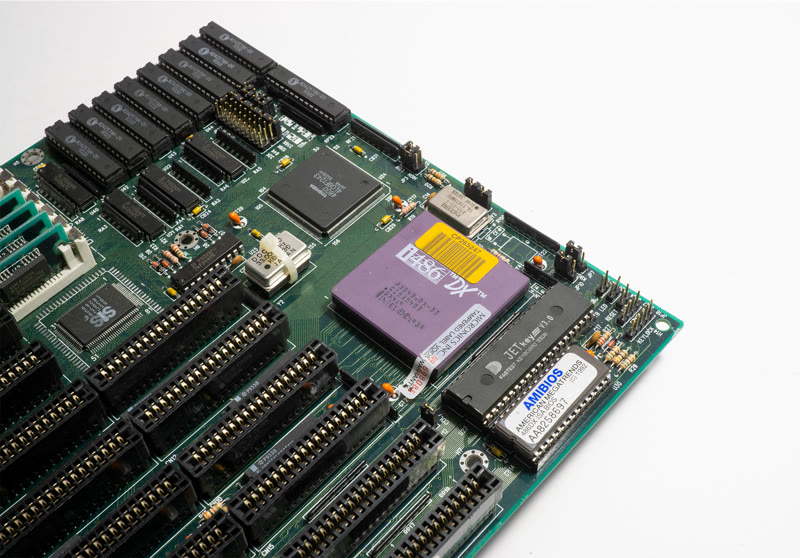
\includegraphics[width=0.5\linewidth]{images/book1/g7-processor-in-socket.jpg}

{\small A \omterm{def:g3:inside-the-computer:processor}{processor} (the purple square) in its socket on an old \omterm{def:g3:inside-the-computer:motherboard}{motherboard}.
Its \omterm{def:g7:how-a-processor-runs-a-program:machine-instruction}{machine language} has well over a hundred \omterm{def:g1:instructions-in-order:instruction}{instructions}.}
\end{omfigure}

\begin{history}[Programs as wiring, then programs in memory]
% ledger: g1:eniac-programming, g7:edvac-1945
ENIAC, the \omterm{def:g1:what-is-a-computer:computer}{computer} of \cref{ch:g1:what-is-a-computer}, kept no \omterm{def:g4:programs-and-operating-system:program}{program} in
its \omterm{def:g3:inside-the-computer:memory}{memory}: its operators set it up for each job by plugging in cables and
setting switches, which could take days. A report dated 30 June 1945, on the
design of its successor EDVAC, described a \omterm{def:g1:what-is-a-computer:computer}{computer} with one large \omterm{def:g3:inside-the-computer:memory}{memory}
holding the \omterm{def:g1:instructions-in-order:instruction}{instructions} as well as the data. Changing the \omterm{def:g4:programs-and-operating-system:program}{program} then meant
changing numbers in \omterm{def:g3:inside-the-computer:memory}{memory}, and almost every \omterm{def:g1:what-is-a-computer:computer}{computer} since has worked that way.
\end{history}

\begin{omfigure}
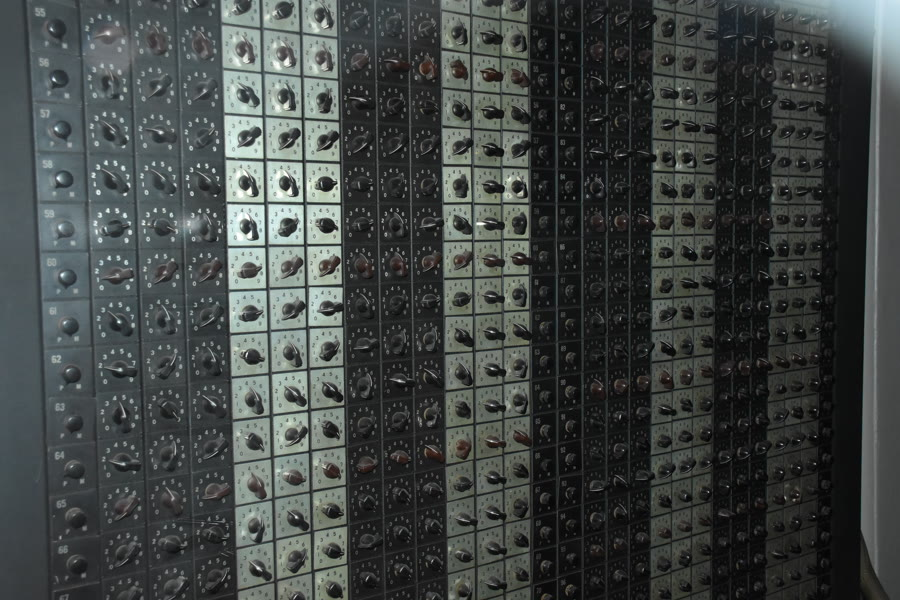
\includegraphics[width=0.55\linewidth]{images/book1/g7-eniac-function-table.jpg}

{\small Rows of hand-set knobs on one of ENIAC's \omterm{def:g7:functions:function}{function} tables, which held
numbers for its calculations.}
\end{omfigure}

\section{Exercises}

\begin{exercise}[$\star$]\label{exo:g7:how-a-processor-runs-a-program:1}
All \omterm{def:g7:how-a-processor-runs-a-program:register}{registers} start at 0. What do \code{R0} and \code{R1} hold when this
\omterm{def:g4:programs-and-operating-system:program}{program} halts?

\omcode{code/grade-7/04-how-a-processor-runs-a-program/exercises/three_steps.toy}{2}{5}{Three
\omterm{def:g1:instructions-in-order:instruction}{instructions}, then \code{HALT}.}\label{lst:g7:how-a-processor-runs-a-program:three-steps}
\end{exercise}

\begin{exercise}[$\star$]\label{exo:g7:how-a-processor-runs-a-program:2}
In \cref{lst:g7:how-a-processor-runs-a-program:sum}, what does \code{PC} hold
after each of the first four steps?
\end{exercise}

\begin{exercise}[$\star$]\label{exo:g7:how-a-processor-runs-a-program:3}
What does \cref{lst:g7:how-a-processor-runs-a-program:countdown} print?
\end{exercise}

\begin{exercise}[$\star$]\label{exo:g7:how-a-processor-runs-a-program:4}
Write a toy \omterm{def:g4:programs-and-operating-system:program}{program} that reads two numbers and prints their sum plus 1.
\end{exercise}

\begin{exercise}[$\star\star$]\label{exo:g7:how-a-processor-runs-a-program:5}
This \omterm{def:g4:programs-and-operating-system:program}{program} should print 3, 2, 1. Here is what happens when it runs; the
machine stops it after 10\,000 steps. What is wrong? Fix it.

\omcode{code/grade-7/04-how-a-processor-runs-a-program/listings/never_ends.toy}{1}{7}{A
countdown that never ends.}\label{lst:g7:how-a-processor-runs-a-program:never-ends}

\omoutput{code/grade-7/04-how-a-processor-runs-a-program/outputs/never_ends_run.txt}{What
it prints is kept in a \omterm{def:g3:files-and-folders:file}{file}; \code{wc -l} counts its lines and \code{tail}
shows the last ones.}\label{out:g7:how-a-processor-runs-a-program:never-ends}
\end{exercise}

\begin{exercise}[$\star\star$]\label{exo:g7:how-a-processor-runs-a-program:6}
Noor forgot the \code{HALT} at the end of
\cref{lst:g7:how-a-processor-runs-a-program:add-two}. Her \omterm{def:g4:programs-and-operating-system:program}{program} still
prints 7 and stops. Why? Why is it still a bug?
\end{exercise}

\begin{exercise}[$\star\star$]\label{exo:g7:how-a-processor-runs-a-program:7}
Write a toy \omterm{def:g4:programs-and-operating-system:program}{program} that prints 5, 4, 3, 2, 1.
\end{exercise}

\begin{exercise}[$\star\star$]\label{exo:g7:how-a-processor-runs-a-program:8}
Using the table of operation codes, write the two \omterm{def:g4:memory-and-storage:byte}{bytes} of
\code{LOADI R1, 7} in decimal and in \omterm{def:g5:bits-and-bytes:binary}{binary}.
\end{exercise}

\begin{exercise}[$\star\star$]\label{exo:g7:how-a-processor-runs-a-program:9}
Without the trace, count the steps that
\cref{lst:g7:how-a-processor-runs-a-program:sum} takes for $n = 4$; then
check your answer on \cref{out:g7:how-a-processor-runs-a-program:sum-trace}.
\end{exercise}

\begin{exercise}[$\star\star\star$]\label{exo:g7:how-a-processor-runs-a-program:10}
The toy \omterm{def:g3:inside-the-computer:memory}{memory} has 256 cells and each \omterm{def:g1:instructions-in-order:instruction}{instruction} takes two. How many
\omterm{def:g1:instructions-in-order:instruction}{instructions} can the longest \omterm{def:g4:programs-and-operating-system:program}{program} have? Why would a real \omterm{def:g4:programs-and-operating-system:program}{program} be
shorter still?
\end{exercise}

\begin{exercise}[$\star\star\star$]\label{exo:g7:how-a-processor-runs-a-program:11}
Find an expression for the number of steps
\cref{lst:g7:how-a-processor-runs-a-program:sum} takes for any $n$, and check
it with a Python \omterm{def:g4:programs-and-operating-system:program}{program} that runs the toy machine for $n = 1$ to 10.
\end{exercise}

\begin{exercise}[$\star\star\star$]\label{exo:g7:how-a-processor-runs-a-program:12}
Write a toy \omterm{def:g4:programs-and-operating-system:program}{program} that reads two numbers below 128 and prints the larger
one. Use \code{CMP} and \code{JN} from the table.
\end{exercise}

\section{Problem: Multiplying on a Machine That Cannot Multiply}

\begin{problem}[{Weekend problem --- multiplying with additions}]\label{pb:g7:how-a-processor-runs-a-program:1}
The toy machine can add and subtract, but it has no \omterm{def:g1:instructions-in-order:instruction}{instruction} to multiply.
Yet $6 \times 4$ is $6 + 6 + 6 + 6$.

\needspace{4\baselineskip}\medskip\noindent\textbf{Part I --- By hand.}
\begin{enumerate}
  \item Write $6 \times 4$ and $4 \times 6$ as sums. Which one has fewer
    additions?
  \item Here is a \omterm{def:g4:programs-and-operating-system:program}{program} that reads $a$ and $b$ and adds $a$ to a total, $b$
    times. Trace it by hand for $a = 6$ and $b = 4$, in a table with the
    columns step, \code{PC}, \code{R0}, \code{R1}, \code{R2}.
\end{enumerate}

\omcode{code/grade-7/04-how-a-processor-runs-a-program/listings/multiply.toy}{1}{10}{Multiplying
by repeated addition.}\label{lst:g7:how-a-processor-runs-a-program:multiply}

\begin{enumerate}[resume]
  \item How many steps did your trace take? Which \omterm{def:g7:how-a-processor-runs-a-program:register}{register} holds the answer?
  \item What does \code{R1} count?
\end{enumerate}

\needspace{4\baselineskip}\medskip\noindent\textbf{Part II --- Counting the steps.}

\omcode{code/grade-7/04-how-a-processor-runs-a-program/listings/multiply_steps.py}{1}{7}{Running
\cref{lst:g7:how-a-processor-runs-a-program:multiply} for $b = 1$ to
10.}\label{lst:g7:how-a-processor-runs-a-program:multiply-steps}

\begin{enumerate}[resume]
  \item Run the \omterm{def:g4:programs-and-operating-system:program}{program}. Does it agree with your trace for $b = 4$?
  \item By how much does the number of steps grow when $b$ grows by 1? Why?
  \item Which steps are done only once, whatever $b$ is? How many are they?
\end{enumerate}

\needspace{4\baselineskip}\medskip\noindent\textbf{Part III --- The cost of a multiplication.}
\begin{enumerate}[resume]
  \item Write the number of steps as an expression in $b$.
  \item Predict the steps for $3 \times 50$ and for $50 \times 3$, then run
    them.
  \item To multiply two numbers, which one should be read second, as $b$?
  \item A \omterm{def:g7:how-a-processor-runs-a-program:register}{register} holds one \omterm{def:g4:memory-and-storage:byte}{byte}, at most 255. What goes wrong with
    $7 \times 200$?
  \item State the result.
\end{enumerate}
\end{problem}
